A projection of a real-world object to an image annihilates its depth
information. This is because the 3D points in the same viewing direction
inherently yield a single 2D point in the image. 3D object scanning and
reconstruction is a technique to acquire enough information in order to
regenerate the 3D shape of such a real-world object. This is achieved by
taking multiple scans of the object from different angles to subsequently
register them in a common coordinate system. The generated 3D models are
widely used for medical diagnosis, achaelogical analysis and documentation,
industrial design and production and in the entertainment industry.

3D scanning techniques can be broadly divided into two categories depending on
whether or not the scanning system is in contact with the target object.  The
contact-free techniques themselves can be either active or passive. Active
contact-free techniques emit a radiation to calculate the deviation from the
object, while passive techniques use the visible light itself for such an
estimation. The authors in \cite{blaisf:2004} provide a solid review of the
most important 3D laser scanning methods developed in the last 20 years.

\begin{figure}[ht!]
\centering
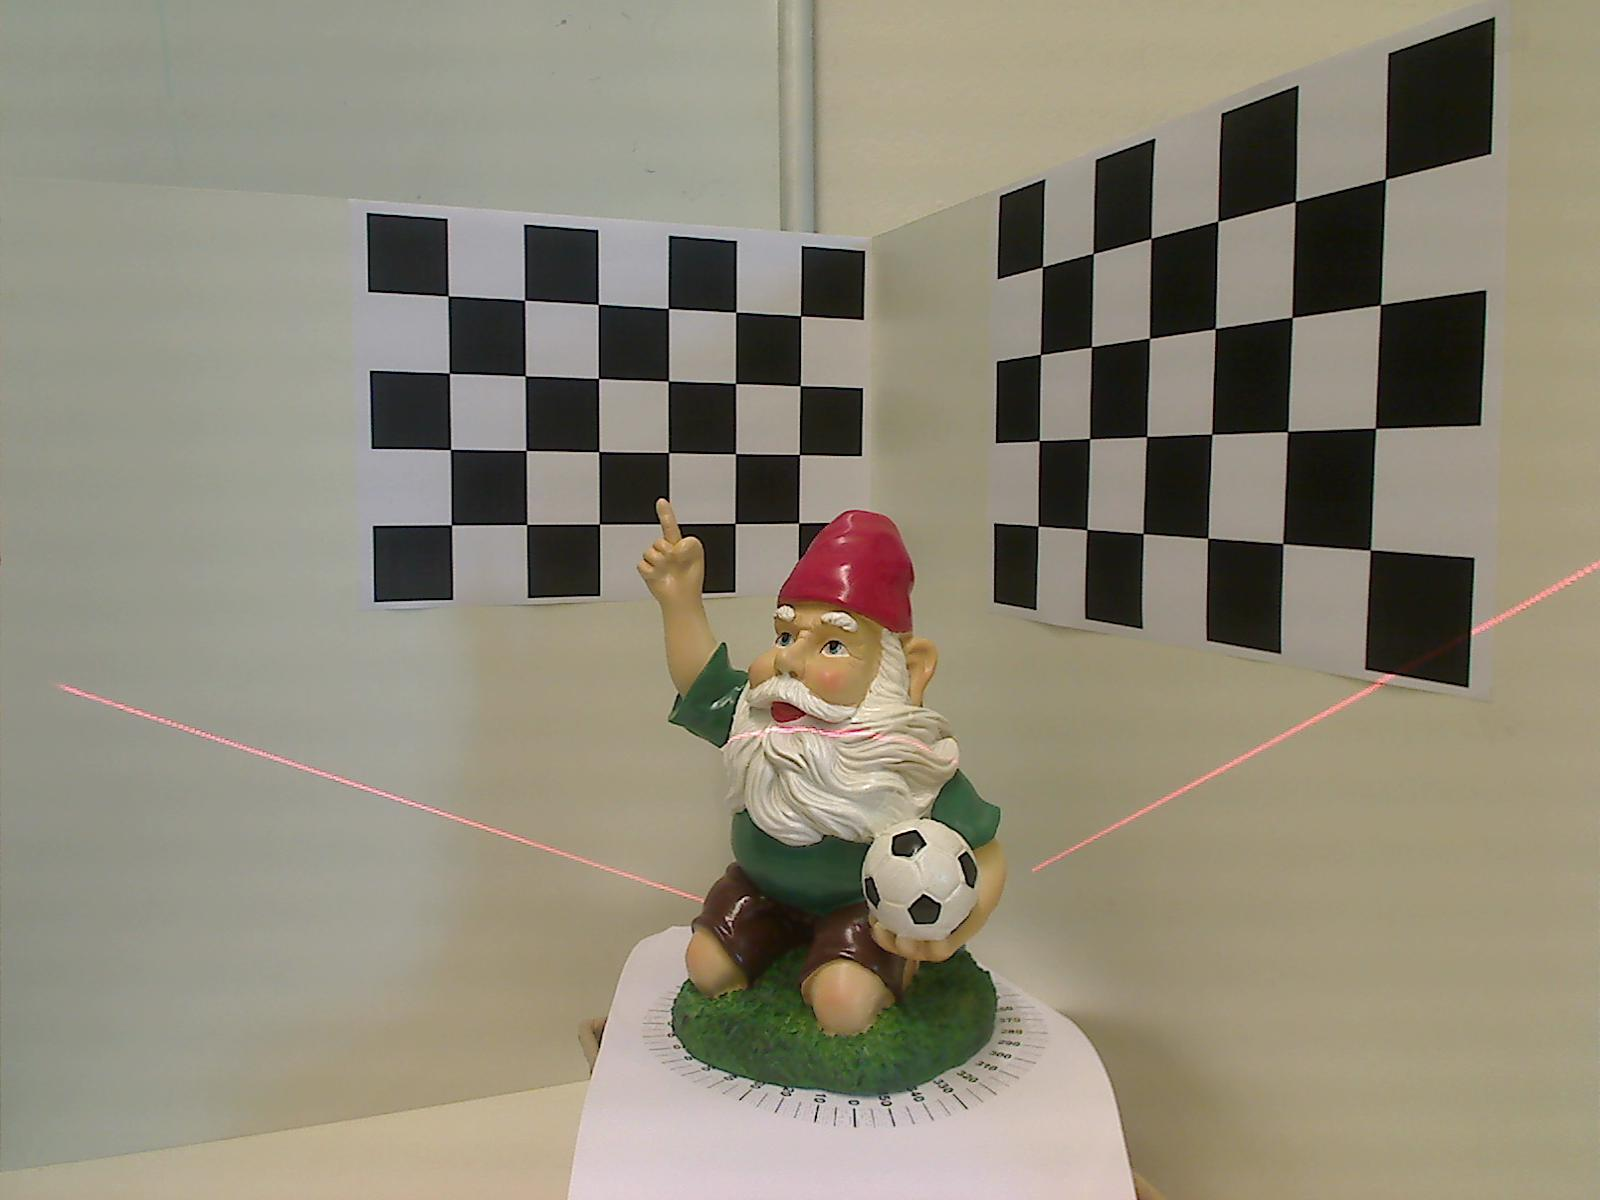
\includegraphics[width=1.00\linewidth]{figures/introduction}
\caption{Data Acquisition Setup}
\label{figure:acquisition}
\end{figure}

This paper uses the active contact-free technique by using a hand-held
projector to emit a laser line. The recovery of the object surface is done by
triangulating the laser with the rays that were projected back to the camera.
We use the real-time self-calibration approach \cite{winkelbach:2006} to
eliminate the need of an external sensor to track the position of the scanner.
The pipeline initially begins with the data acquisition using an inexpensive
web camera that captures multiple runs of a laser sweeping across an object as
shown in figure \ref{figure:acquisition}. Camera calibration using a
chessboard pattern is performed next, that helps estimate the internal
parameters of the camera to establish a mapping between its natural units to
the units in the physical world. We also use the chessboard patterns as our
reference double-frames to calculate the extrinsic parameters of the camera.
These parameters are later used to calculate the pose\footnote{combination of
position and orientation} of the laser plane.

The quality of the final 3D shape depends largely on how accurately the laser
lines and the object points are identified. We use a reference image without a
laser line to calculate an image difference with each frame of the laser
sweeping the object as used in \cite{winkelbach:2006}. The difference image is
then smoothened and filtered with a red color threshold to remove the
outliers. Hough transform on the result helps isolate the two laser lines on
each side of the object from the object points.

The extrinsic parameters of the camera calculated using the chessboard
patterns are used with the laser pixels from the hough lines to calculate the
laser plane equation. The laser plane equation is finally intersected with the
object points to determine the 3D surface points (point cloud) of the objects.
The point clouds from each scan (with a different orientation of the object)
are registered using \ac{ICP} \cite{besl:1992}. We use \ac{SLAM} from
\ac{3DTK} \cite{3dtk:2012} for automatic scan registration.

